\documentclass[11pt,a4paper]{article}

% Packages
\usepackage{graphicx}                 
\usepackage{hyperref}                
\usepackage{cite}
\usepackage[latin1]{inputenc}
\usepackage{geometry}
\geometry{margin=1in}                  
\usepackage{tikz}
\usetikzlibrary{positioning}
\usepackage{algorithmic} 
\usepackage{glossaries}  

\makeglossaries

% Glossary entries
\newglossaryentry{host}{
    name=Host,
    description={In SimGrid, represents a resource of computational power (e.g., CPU, GPU, one CPU core...)}
}

\newglossaryentry{activity}{
    name=Activity,
    description={In SimGrid, an activity is an elemental action of the system. 
    Example: a communication between two Hosts, a computation on one Host, a write on a Disk...}
}

\newglossaryentry{actor}{
    name=Actor,
    description={A SimGrid actor represents the process to simulate. It can interact
     with the system by launching activities, suspending actors, killing actors, shutting 
     down Hosts...}
}



\begin{document}

\begin{titlepage}
    \centering
    \vspace*{2cm}
    \Huge
    \textbf{Simulation of NCCL with SimGrid}
    
    \vspace{0.5cm}
    \Large
    Jean Conan \\
    TU Wien
    
    \vfill
    \Large
    \textbf{Technical Report} \\
    \vspace{0.5cm}
    \today
    \vspace{2cm}
\end{titlepage}

\maketitle

% Abstract
\begin{abstract}
This article demonstrates how GPU-to-GPU communications can be modeled using SimGrid by 
implementing a subset of the CUDA Runtime Library and NCCL with SimGrid's high-level interface (s4u).
\end{abstract}

\textbf{Keywords:} GPU communication, SimGrid, CUDA Runtime, NCCL, Simulation

\section{Introduction}
GPUs play a crucial role in modern high-performance computing (HPC) systems, and efficient 
communication between them is critical for performance. The NCCL (NVIDIA Collective Communications Library) 
is widely used for optimized multi-GPU communications. In this report, we demonstrate how GPU-to-GPU 
communications can be modeled using SimGrid \cite{simgrid}, a simulation framework, by implementing a subset of the 
CUDA Runtime Library \cite{cudart} and NCCL \cite{nccllib}.

The objective of this work is to assess the feasibility of SimGrid in modeling NCCL and CUDA features for GPU communication. We present the methodology, implementation details, and preliminary results based on simulations of real-world communication patterns.


\printglossary

\section{Methodology}
In this section, we describe the methods used to simulate GPU communication 
using SimGrid, covering both the theoretical and practical aspects. We detail 
the modeling of GPUs, the integration of CUDA Runtime features, and the extension 
of SimGrid to support NCCL communication primitives.

\subsection{Modeling a General-Purpose GPU}
\subsubsection{SimGrid Philosophy}
SimGrid uses a resource-based logic to describe hardware. CPUs are typically 
modeled by computational power resources (s4u Hosts), and interconnection 
links are modeled by bandwidth resources (s4u Links).

It is logical to model a GPU as a \gls{host}, as it is also a computational 
resource. What differentiates a CPU from a GPU is how they interact with 
resources. A simulated CPU algorithm (s4u Actor) launches \glspl{activity} 
on the host it is located on, while a simulated GPU algorithm is run on a 
CPU, which then launches \glspl{activity} on the associated GPUs.

\subsubsection{A Stream-Controlled \gls{host}}
Using SimGrid's extension mechanism, a queue of "kernel calls" is linked to a 
simple \gls{actor} called the "Stream Actor". The Stream Actor behaves as follows:

\begin{algorithmic}
    \WHILE{true}
        \IF{stream is empty}
            \STATE suspend
        \ELSE
            \STATE kernel = stream.pop()
            \STATE consume(kernel)
        \ENDIF
    \ENDWHILE
\end{algorithmic}

When a new kernel call is added by the CPU \gls{actor} that created the stream, 
it resumes the stream \gls{actor}, which then consumes all kernel calls. Consuming 
a kernel call means translating it into \glspl{activity} on the GPU and waiting 
for these \glspl{activity} to complete.

\subsection{CUDA Runtime Library}
NCCL-tests (a collection of tests for NCCL) use a small portion of the CUDA Runtime 
Library, primarily stream management and synchronization. The most recent version 
also uses CUDA Graphs.

\subsubsection{Stream Management and Synchronization}
The most important functions to cover are:
\begin{itemize}
    \item \texttt{cudaSetDevice(int device)}
    \item \texttt{cudaStreamCreateWithFlags(cudaStream\_t *pStream, unsigned int flags)}
    \item \texttt{cudaStreamSynchronize(void)}
\end{itemize}

The first two functions create a Stream object associated with a GPU. In the 
\texttt{cudaStreamCreateWithFlags} call, there is no option to specify which 
GPU \gls{host} to use, so a SimGrid extension is used to store the GPU \glspl{host} 
accessible by the CPU. The \texttt{cudaStreamSynchronize} function allows the CPU 
to wait for all kernels to finish on the GPU. In the implementation, the CPU probes 
the stream actor to check if it is suspended, and if it isn't, it suspends itself.

Other CUDA Runtime functions used by NCCL-tests include \texttt{cudaMalloc}, 
\texttt{cudaHostMalloc}, \texttt{cudaHostFree}, \texttt{cudaFree}, and \texttt{cudaMemcpy}.

\subsubsection{CUDA Graphs}
In the most recent NCCL-tests, CUDA Graphs are utilized. A CUDA Graph is a set 
of kernels that can be launched together and multiple times. This mechanism has 
advantages such as easier communication of kernel calls to the GPU and simplifying 
the repeated launch of the same kernel.

There are two main objects: \texttt{CudaGraph} and \texttt{CudaGraphExec}. A 
\texttt{CudaGraph} can be modified, while a \texttt{CudaGraphExec} can be launched. 
In NCCL-tests, CUDA Graphs are created using the capture method: first, 
\texttt{cudaStreamBeginCapture} is called, then all the kernel calls are issued, 
followed by \texttt{cudaStreamEndCapture}. Afterward, the \texttt{CudaGraph} is 
converted into a \texttt{CudaGraphExec} using \texttt{cudaGraphInstantiate}, and 
it is launched with \texttt{cudaGraphLaunch}.

To implement this, a high-level stream object was created. If there is no capture, 
it passes activities to the lower-level stream; if in capture mode, it adds the 
activities to the graph.

Since CUDA Graphs are essentially graphs of kernels, and kernels are graphs of 
activities in our simulation, CUDA Graphs can be represented as graphs of activities. 
However, CUDA Graphs can be launched multiple times, and kernels may involve 
data-dependent operations, requiring activities to be computed in the simulation as well.

To address this, a structure called \texttt{GpuActivity} was created. Alternatively, 
an extension of s4u Tasks could have been used.

\subsection{NCCL}
\subsubsection{Communicators and Basic Communication}
NCCL communicators are objects used for every communication. They are created from a 
unique ID. In NCCL, the ID is a constant-length string, but in the simulated library, 
an integer is used for simplicity. To create a communicator with multiple CPUs, one CPU 
generates the unique ID and broadcasts it to the others.

In the simulated implementation, \texttt{ncclComm} points to an object that holds a 
mapping of ranks to GPUs.

\subsubsection{Collectives}
NCCL collectives have been implemented as kernels, using \texttt{ncclGroup}, 
\texttt{ncclSend}, and \texttt{ncclRecv}. NVIDIA's documentation on communication 
patterns was partial, so additional information was obtained from third-party sources.

\subsection{SMPI}
The simulation library can be used with SMPI, for example, to communicate 
\texttt{ncclUniqueId} to create a common communicator with multiple CPUs. One issue 
that may arise is deadlock detection: if all processes involved in the SMPI 
application get suspended, an SMPI internal mechanism triggers a deadlock error, even 
if there isn't one (e.g., when all CPUs are waiting for corresponding GPUs for 
synchronization). To avoid this, a blank SMPI process can be added to wait on a final 
barrier before calling \texttt{MPI\_Finalize} and exiting.

\section{Experiments}
NCCL-tests were run on Tesla GPUs, and the AMD equivalent RCCL-tests were run on 
MI100 GPUs on the Chameleon Cloud. Only one node and two GPUs were used for each test, 
so comparison at scale between reality and simulation has not been evaluated.

A simple model for a single node with two GPUs is illustrated as follows:

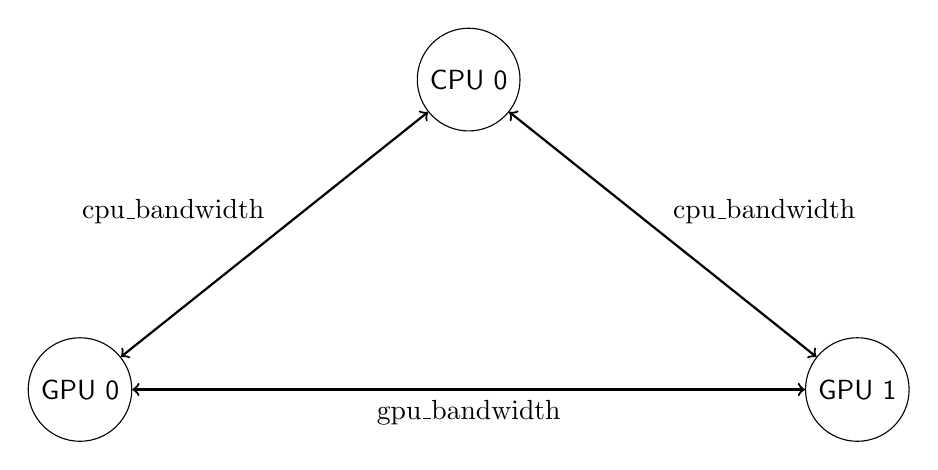
\begin{tikzpicture}[
    node distance=3cm and 4cm, 
    main/.style = {draw, circle, minimum size=1cm, text centered, font=\sffamily}
]

\node[main] (cpu0) {CPU 0};
\node[main, below left=of cpu0] (gpu0) {GPU 0};
\node[main, below right=of cpu0] (gpu1) {GPU 1};

\draw[<->, thick] (cpu0) -- node[midway, above left] {cpu\_bandwidth} (gpu0);
\draw[<->, thick] (cpu0) -- node[midway, above right] {cpu\_bandwidth} (gpu1);
\draw[<->, thick] (gpu0) -- node[midway, below] {gpu\_bandwidth} (gpu1);

\end{tikzpicture}

The measured bandwidth for NCCL communications corresponds to the GPU bandwidth. For 
communications other than AllReduce, Reduce, and ReduceScatter, the computational power 
of the GPU plays no role, and the CPU-to-GPU bandwidth only matters for very small 
communication sizes (comparable to kernel call sizes).

\section{Conclusion}
In this report, we have demonstrated that SimGrid can successfully model GPU-to-GPU 
communications using NCCL and the CUDA Runtime Library. While the experiments presented 
here focus on a small-scale simulation, the approach can be extended to larger systems. 
The ability to model detailed communication and computational behavior of GPUs in SimGrid 
opens up possibilities for performance prediction and optimization in HPC systems.

\subsection{Future Work}
Future work could include:
\begin{itemize}
    \item Extending the model to support Hip Runtime (for AMD GPU).
    \item Add in place collectives support
    \item Adding a snvcc compiler to function like \texttt{smpi\_cc} for \texttt{mpi\_cc} : compiling native code directly into SimGrid.
    \item Evaluating the performance of other NCCL collectives at scale.
    \item Incorporating more detailed performance metrics for comparison with real-world results.
\end{itemize}


\bibliographystyle{plain}
\bibliography{bib.bib}
\end{document}
